\documentclass[11pt,spanish]{article}

% Paquetes
\usepackage{amstext}
\usepackage{amssymb}
\usepackage{amsmath}
\usepackage{babel}
    \addto\shorthandsspanish{\spanishdeactivate{~<>}}
    \decimalpoint
\usepackage[style=iso]{datetime2}
\usepackage{fancyhdr}
\usepackage{float}
\usepackage[T1]{fontenc}
\usepackage[a4paper]{geometry}
    \geometry{verbose,tmargin=3cm,bmargin=2cm,lmargin=2.5cm,rmargin=2.5cm}
\usepackage{graphicx}
\usepackage{hyperref}
\usepackage[utf8]{inputenc}
\usepackage{lastpage}
\usepackage{mathptmx}
\usepackage{tasks}
\usepackage{units}
\usepackage{siunitx}

% dibujos 

\usepackage{tikz}
\usepackage{tikz-dimline}
\usetikzlibrary{calc}
% \usetikzlibrary{math}
\usetikzlibrary{arrows.meta}
\usetikzlibrary{snakes}
\usetikzlibrary{decorations}
\usetikzlibrary{decorations.pathmorphing}
\usetikzlibrary{patterns}

% tipo de fuente 
\usepackage{lmodern}

\pagestyle{fancy}
\lfoot{\small DF, FCEyN, UBA}
\cfoot{\tiny Actualizado el {\today} a las {\DTMcurrenttime}}
\rfoot{\small Pág. {\thepage} de \pageref{LastPage}}

\begin{document}

% Título
    \begin{center}
    \textsc{\large Física 2 (Física) - Cátedra Diana Skigin}
    \par\end{center}{\large \par}
    
    \begin{center}
    \textsc{\large Segundo Cuatrimestre de 2021}
    \par\end{center}{\large \par}
    
    \begin{center}
    \textsc{\large Guía 6: Paquetes de Ondas}
    \par\end{center}{\large \par}

% Comienzo 
\begin{enumerate}

\section*{Velocidad de grupo y de fase}

% Ejercicio 1

    \item Discuta cuál de estos métodos permite determinar
    la velocidad de fase y cuál la de grupo:

    \begin{enumerate}
        \item Medir la velocidad del sonido en el aire, golpeando las manos y
        determinando el tiempo que transcurre entre el aplauso y el eco de un
        reflector ubicado a una distancia conocida.

        \item Medir la longitud de un tubo que resuena a una frecuencia conocida
        (y corregir por efectos de borde).

        \item Determinar la velocidad de la luz midiendo el tiempo que tarda un
        haz colimado en recorrer una distancia conocida.

        \item Encontrar la longitud de una cavidad resonante que oscila en un
        modo conocido a una frecuencia conocida.
    \end{enumerate}

% Ejercicio 2

    \item Obtenga la velocidad de fase y de grupo para los siguientes casos.
    Compárelas y discuta para cuales ambas son similares.
    
    \begin{enumerate}
        \item Ecuación de ondas clásica.
        \item Ecuación de Klein-Gordon, considerando las siguientes situaciones:
        \begin{enumerate}
            \item $\omega_0 = 0$, con $c$ y $k_0$ arbitrarios.

            \item $\omega_0 = \SI{1}{\per\second}$ y $c=\SI{1}{\meter\per\second}$,
            con $k_0$ tomando los valores: $\SI{1}{\per\meter}$,
            $\SI{3}{\per\meter}$, y $\SI{10}{\per\meter}$.
        \end{enumerate}
    \end{enumerate}

% Ejercicio 3

    \item Demuestre que la velocidad de grupo $v_\text{g}$ y la velocidad de fase
    $v_\text{f}$ están relacionadas por:
    \[
    v_\text{g}=v_\text{f}-\lambda\frac{dv_\text{f}}{d\lambda}
    \]
    ¿Cómo es $\frac{dv_\text{f}}{d\lambda}$ en un medio no dispersivo? En
    ese caso, ¿cómo se relacionan la velocidad de grupo y la de fase?


\section*{Paquetes Gaussianos}

% Ejercicio 4

    \item \textbf{Función Gaussiana:} Considere la siguiente función de una
    coordenada arbitraria $z$:
    \[
    F(z)=A\exp\left[-\frac{(z-\mu)^{2}}{4\Delta ^{2}}\right],
    \]
    conocida como función de Gauss (\textit{aka} campana de Gauss, función
    normal, etc.), cuyos parámetros $A$, $\mu$ y $\Delta$ son conocidos.
    
    \begin{enumerate}
        \item Muestre analítica o gráficamente que esta función:
        \begin{itemize}
            \item es definida positiva.
            \item tiene un único máximo en $z = \mu$.
            \item tiende a $0$ para $z \to \pm \infty$.
        \end{itemize}
 
        \item Determine el desplazamiento en $z$ respecto a la posición del
        máximo, necesario para que la altura de la función se reduzca a la
        mitad. Es decir, obtenga $\Delta z$ tal que:
        $$F(z \pm \Delta z)=\nicefrac{1}{2} F(\mu)$$
        Utilice este resultado para definir el ancho de la campana. ¿Qué
        parámetro de la función determina dicho ancho?
        
        \item ¿A qué altura de la función corresponde el ancho definido por
        $2 \Delta$?
    \end{enumerate}

% Ejercicio 5

    \item Se quiere investigar la relación entre el ancho de un paquete y el
    desfasaje de las frecuencias que lo componen.

    \begin{enumerate}

        \item Tome el siguiente pulso con un espectro gaussiano de ancho $\Delta k$
        centrado en $k_{0}$ (note que las frecuencias están en fase):
        \[
        F(k)=A\exp\left[-\frac{(k-k_{0})^{2}}{4\Delta k^{2}}\right].
        \]
        Calcule $f(x)$ y vea que tiene una envolvente gaussiana que modula
        una portadora de frecuencia $k_{0}$. Note que el pulso está centrado
        en $x=0$ y que se cumple la relación $\Delta x\Delta k=\nicefrac{1}{2}$
        (el paquete Gaussiano es el de mínima incerteza).

        \item Ahora desfase las distintas frecuencias en forma lineal, tal que:
        \[
        F(k)=A\exp\left[-\frac{(k-k_{0})^{2}}{4\Delta k^{2}}\right]\exp\left[i\alpha(k-k_{0})\right].
        \]
        Calcule $f(x)$ y vea que es el mismo pulso que en la parte (a), pero
        desplazado en $\alpha$ hacia la derecha (una fase lineal sólo corre
        la función).

        \item Ahora agregue una fase cuadrática, es decir:
        \[
        F(k)=A\exp\left[-\frac{(k-k_{0})^{2}}{4\Delta k^{2}}\right]\exp\left[i\beta(k-k_{0})^{2}\right].
        \]
        Calcule $f(x)$ y vea que es un pulso gaussiano centrado en $x=0$
        pero con un ancho $\Delta x$ que cumple:
        \[
        \Delta x\Delta k=\frac{1}{2}\sqrt{1+16\beta^{2}\Delta k^{4}}.
        \]
        
        Verifique que esta relación cumple la relación de incerteza general
        $\Delta x \Delta k \geq \nicefrac{1}{2}$, y luego determine el valor de
        $\beta$ tal que se cumpla la relación de mínima incerteza
        $\Delta x \Delta k = \nicefrac{1}{2}$.
        
        \item A partir del resultado anterior, discuta si es cierto que, si se
        quiere disminuir el ancho de un paquete ($\Delta x$), \textit{siempre}
        se debe aumentar el ancho de su espectro ($\Delta k$). ¿Contradice esto
        a la relación de incerteza mínima?

        \textbf{Sugerencia:} Puede ser útil obtener $\Delta x$ como función de
        $\Delta k$, y luego graficar o derivar la primera en función de la
        segunda.

    \end{enumerate}

    \begin{description}
        \item [{Ayuda:}] $\int_{-\infty}^{+\infty}\exp\left[(x+a)^{2}\right]dx=\sqrt{\pi}$.
    \end{description}

% Ejercicio 6

    \item Repita el ejercicio anterior considerando que el espectro $F(k)$
    corresponde a un pulso que se propaga en un medio arbitrario en $t=0$.
    Resuelva analíticamente a partir de la linealización de la relación de
    dispersión y halle $\Psi(x,t)$ en cada caso. ¿Qué supuestos debe verificar
    el espectro para que el desarrollo sea lo más exacto posible?

% Ejercicio 7

    \item Se tiene un pulso de ancho $\Delta k$ centrado en $k_{0}$ tal que
    la siguiente es una buena aproximación para la relación de dispersión:
    \[
    \omega(k)=\omega_{0}(k_{0})+\omega'(k_{0})(k-k_{0})+\frac{1}{2}\omega''(k_{0})(k-k_{0})^{2}
    \]
    Si en $t=0$ el pulso se propaga hacia $x<0$, y se escribe:
    \[
    \Psi(x,0)=A\int_{-\infty}^{+\infty}\exp\left[-\frac{(k-k_{0})^{2}}{4\Delta k^{2}}\right]\exp\left(ikx\right)dk+ \text{c.c.}
    \]
    Calcule $\Psi(x,t)$. Vea cuál es la posición y el ancho del paquete
    como función del tiempo. ¿Es cierto que al viajar por un medio dispersivo
    cualquier paquete se ensancha?


\section*{Propiedades de la transformada de Fourier}    
    
% Ejercicio 8    
    
    \item Sea $\phi(t)$ una función real. Muestre que su transformada de Fourier
    $\Psi(\omega)$ cumple $\Psi(\omega)=\Psi(-\omega)$. Use esto para escribir a
    $\phi(t)$ como superposición de senos y cosenos.

% Ejercicio 9        

    \item Muestre que la transformada de Fourier $\mathcal{F}$ es lineal, esto
    quiere decir que
    \[
    \mathcal{F}(af+bg)=a\mathcal{F}(f)+b\mathcal{F}(g)
    \]
    donde $f$ y $g$ son funciones de $x$, y donde $a$ y $b$ son constantes.


\section*{Paquetes cuadrados}

% Ejercicio 10

    \item Si $\Psi(\omega)$ corresponde a un espectro de frecuencias cuadrado,
    o sea $\Psi(\omega)=1/\Delta\omega$ para $\omega$ comprendida en
    el intervalo de ancho $\Delta\omega$ alrededor de $\omega_{0}$,
    y cero en otra parte; vea que $\phi(t)$ está dada por: 
    \[
    \phi(t)=\frac{1}{\sqrt{\pi}}\left[\frac{\sin(t\Delta\omega/2)}{t\Delta\omega/2}\right]e^{i\omega_{0}t}
    \]

    \begin{enumerate}
        \item Grafique $\Psi(\omega)$ y $\left|\phi(t)\right|$.

        \item Sea $T$ un tiempo más prolongado que la duración de cualquier
        experimento que pueda idear. Muestre que si $\Delta\omega$ es
        suficientemente pequeño como para que $\Delta\omega T\ll1$, entonces
        durante un tiempo menor que $T$, $\phi(t)$ es una función armónica de
        amplitud y fase casi constante.
    \end{enumerate}

% Ejercicio 11

    \item Considere una pulsación que se repite $N$ veces en el tiempo, dando
    lugar a la siguiente señal $\phi$:

    \begin{figure}[H]
        \centering{}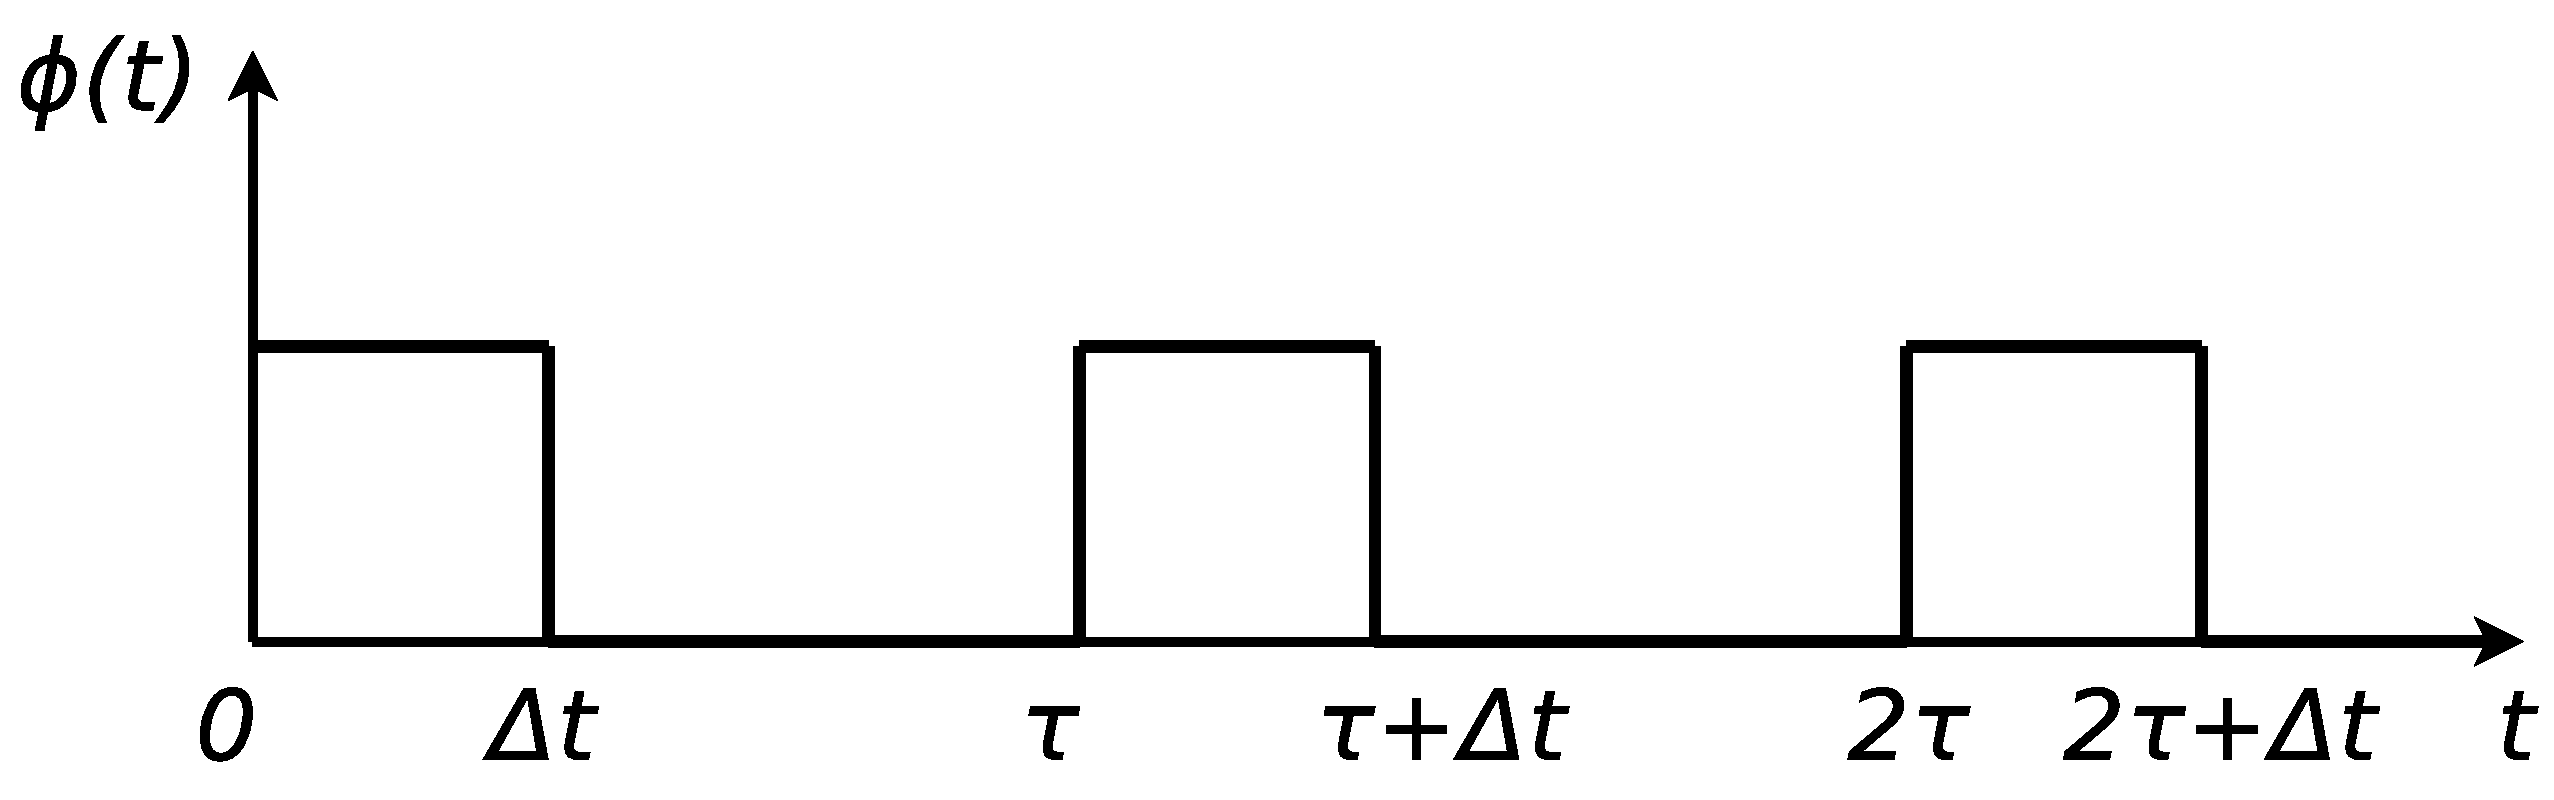
\includegraphics[clip,scale=0.25]{figs/ej2-18}
    \end{figure}

    \begin{enumerate}
        
        \item Vea que la transformada de Fourier de un único pulso situado en el
        intervalo $(n\tau,n\tau+\Delta t)$ es igual a la transformada del pulso
        situado en $(0,\Delta t)$, multiplicado por la fase $e^{in\phi}$.
        Calcule entonces la transformada de la pulsación cuadrada que se repite
        en un tiempo largo $T_\text{largo}=N\tau$.

        \item Muestre que, para un valor finito de $T_\text{largo}$, el análisis
        de Fourier de esta pulsación cuadrada repetida casi periódicamente,
        consiste en una superposición de armónicos casi discretos de la
        frecuencia fundamental $\nu_{1}=1/T_{1}$, siendo realmente cada armónico
        un continuo de frecuencias que se extiende sobre una banda de ancho
        $\delta\nu\approx1/T_\text{largo}$. Los componentes armónicos más
        importantes caen entre 0 y $\Delta\nu=1/\Delta t$.

        \item ¿Por qué vale $\Delta t\Delta\nu\approx1$ si, en principio, podría
        valer $\Delta t\Delta\nu\gg1$? ¿La misma pregunta es aplicable a
        $\delta\nu$ y $T_\text{largo}$?
    \end{enumerate}


\section*{Propagación de paquetes en interfaces}

% Ejercicio 12

	\item Se tienen dos cuerdas semi--infinitas de distinta densidad lineal
	de masa, $\mu_{1}$ y $\mu_{2}$, unidas en un punto y sometidas
	a una tensión $T_0$. Sobre la primera, se propaga hacia la derecha una
	perturbación de la forma indicada en la figura, a velocidad $v$. Se conocen
    $\mu_{1}$, $\mu_{2}$, $T_0$, $L$ y $h$.

	\begin{figure}[H]
		\centering{}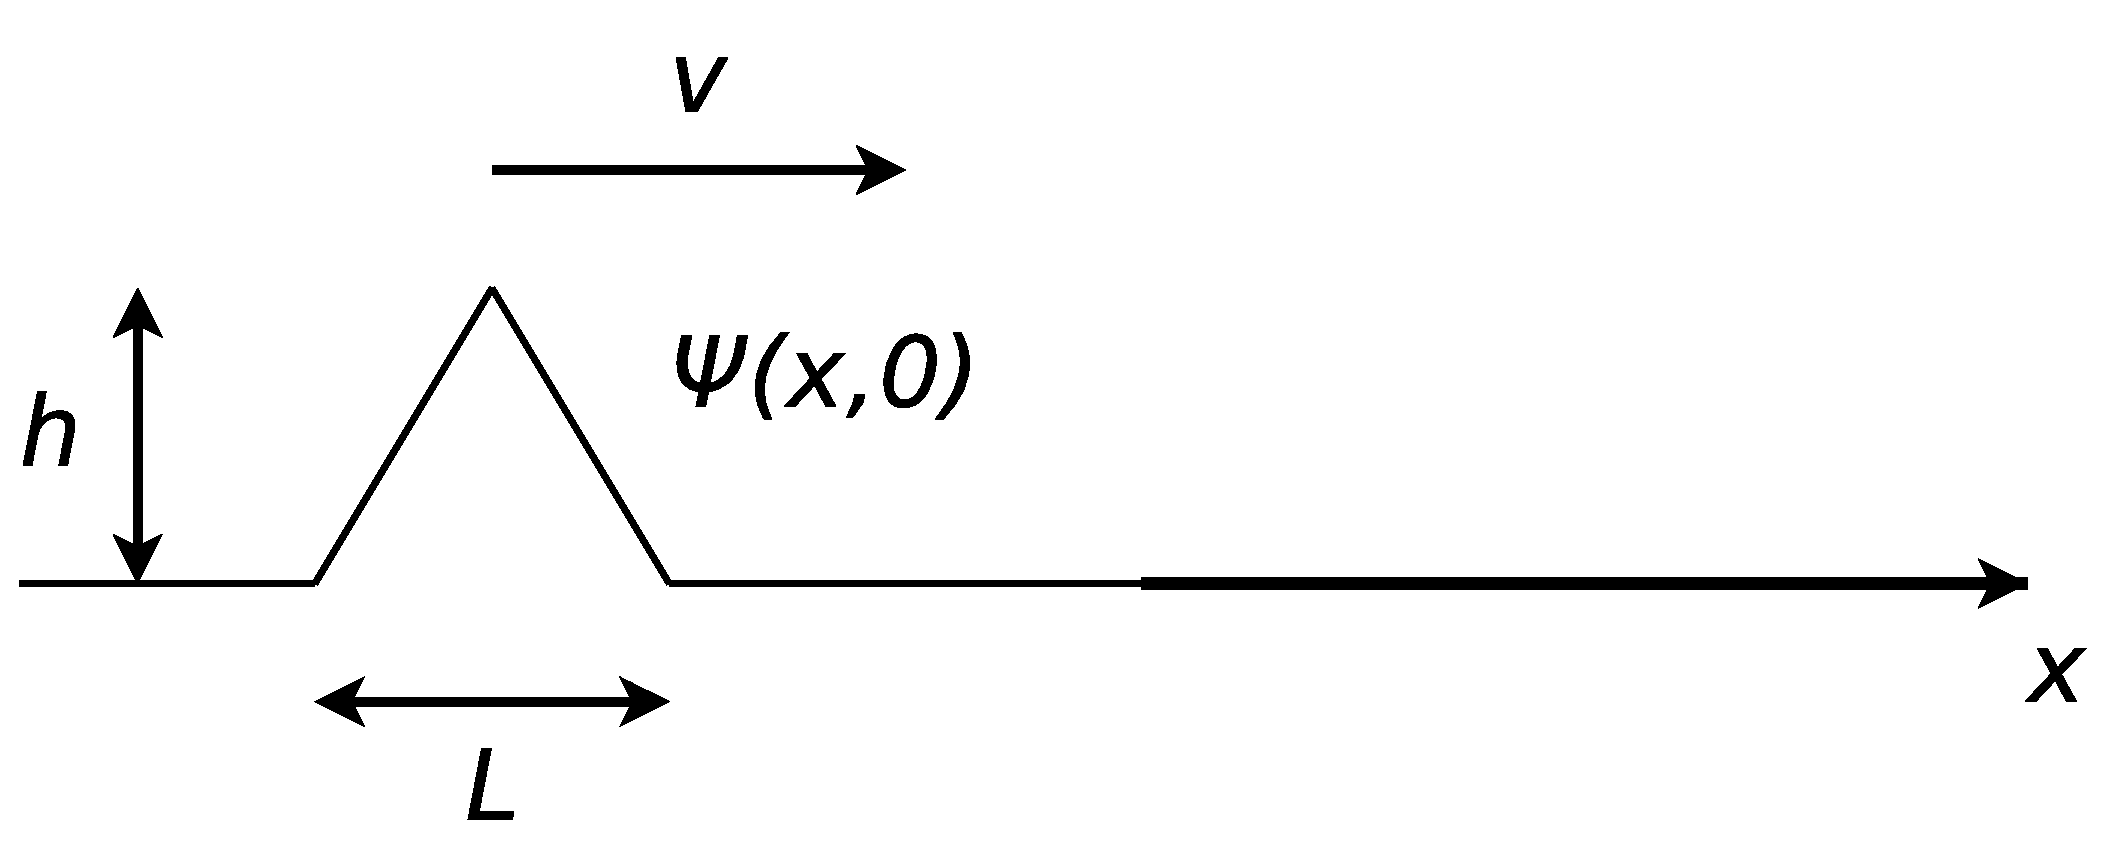
\includegraphics[clip,scale=0.25]{figs/ej2-20}
	\end{figure}

	\begin{enumerate}
		\item Hallar el desplazamiento $\Psi(x,t)$ considerando que los medios
    	son no dispersivos.

		\item Explique cualitativamente cómo cambian estos resultados si el
        segundo medio es dispersivo.
	\end{enumerate}
    
\end{enumerate}

\end{document}
